\appendix

\section{Additional Results}
\label{app:results}

\textbf{t-SNE comparison (EquiSSL-perm vs.\ SANE).}
Figures~\ref{fig:tsne_seed0_equi} and~\ref{fig:tsne_seed0_sane} show the distributional
contrast between EquiSSL-perm and SANE latent spaces in full detail.
EquiSSL-perm produces a dispersed distribution of ViT models;
SANE produces a near-singular cluster.

\begin{figure}[h]
  \centering
  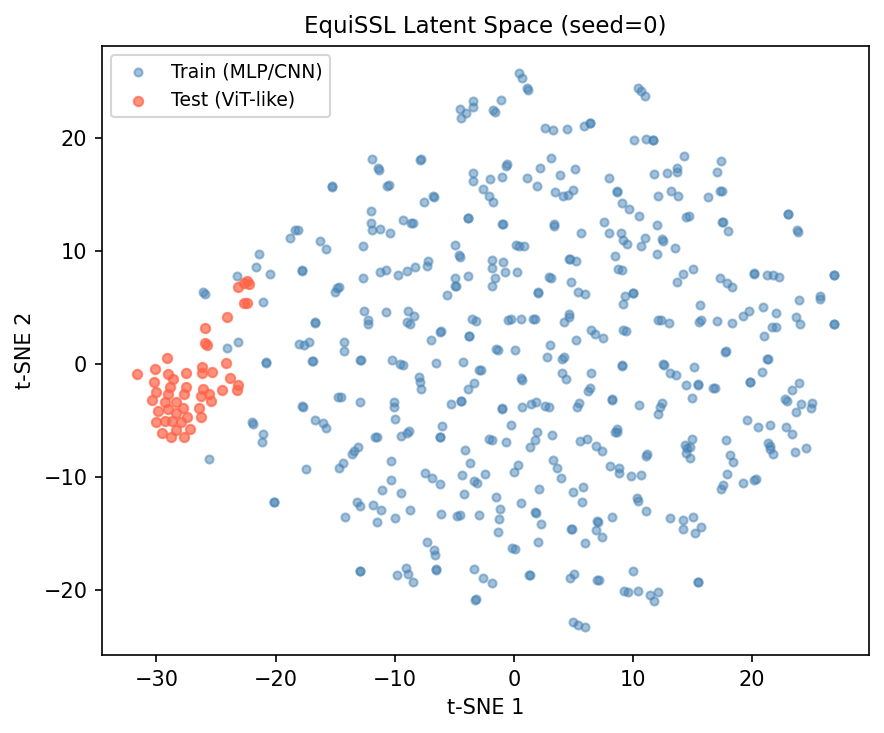
\includegraphics[width=0.7\linewidth]{figures/tsne_equissl_seed0.png}
  \caption{EquiSSL-perm t-SNE latent space (seed 0).
           ViT models are well-distributed across the latent space.}
  \label{fig:tsne_seed0_equi}
\end{figure}

\begin{figure}[h]
  \centering
  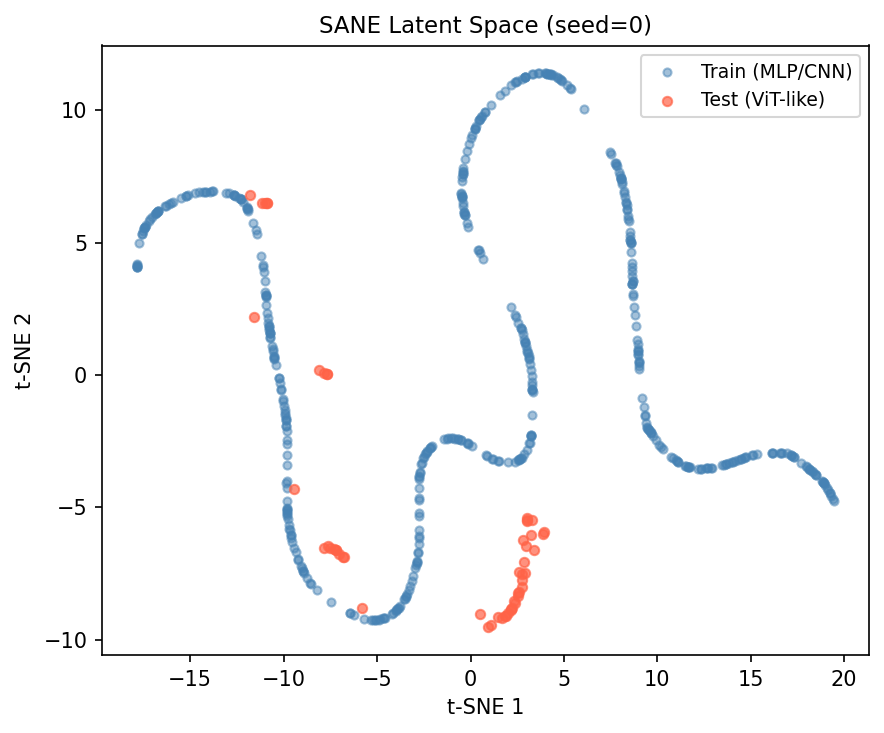
\includegraphics[width=0.7\linewidth]{figures/tsne_sane_seed0.png}
  \caption{SANE t-SNE latent space (seed 0).
           All ViT models collapse to a near-singular cluster ($\text{std} \approx 0.0014$).}
  \label{fig:tsne_seed0_sane}
\end{figure}

\textbf{Latent interpolation failure.}
Figure~\ref{fig:delta_full} shows the full distribution of
$\text{acc}_\text{latent} - \text{acc}_\text{ws}$ across all 501 model pairs,
confirming the consistently negative delta and 90.6\% failure rate.

\begin{figure}[h]
  \centering
  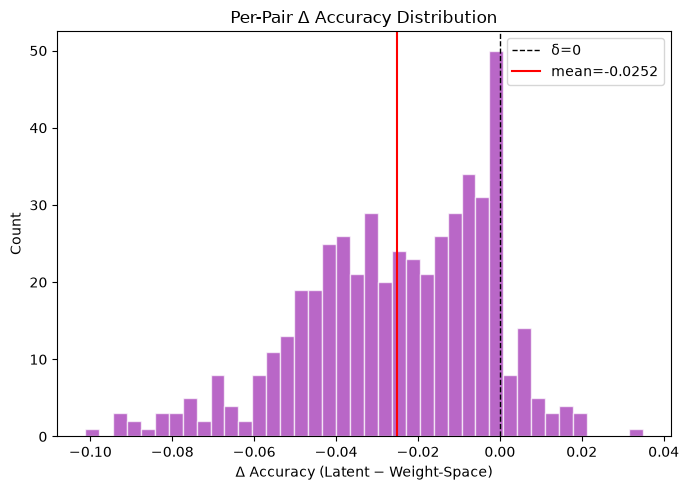
\includegraphics[width=0.6\linewidth]{figures/delta_histogram.png}
  \caption{Full distribution of $\text{acc}_\text{latent} - \text{acc}_\text{ws}$
           over 501 model pairs.
           Strongly left-skewed, centered at $-0.025$, with only 9.4\% positive values.}
  \label{fig:delta_full}
\end{figure}

\textbf{MMD comparison.}
Figure~\ref{fig:mmd_app} shows the MMD measurement results side-by-side for SANE and
EquiSSL.
Note that this figure contains only the two methods for which cross-architecture MMD
(CNN train zoo $\to$ ViT test zoo) was measured.
EquiSSL-perm is not included because cross-architecture MMD was not computed in h-e1;
h-m2 reports only within-ViT-zoo subpopulation MMD for EquiSSL-perm (0.203),
which is a different quantity and cannot be directly compared.

\begin{figure}[h]
  \centering
  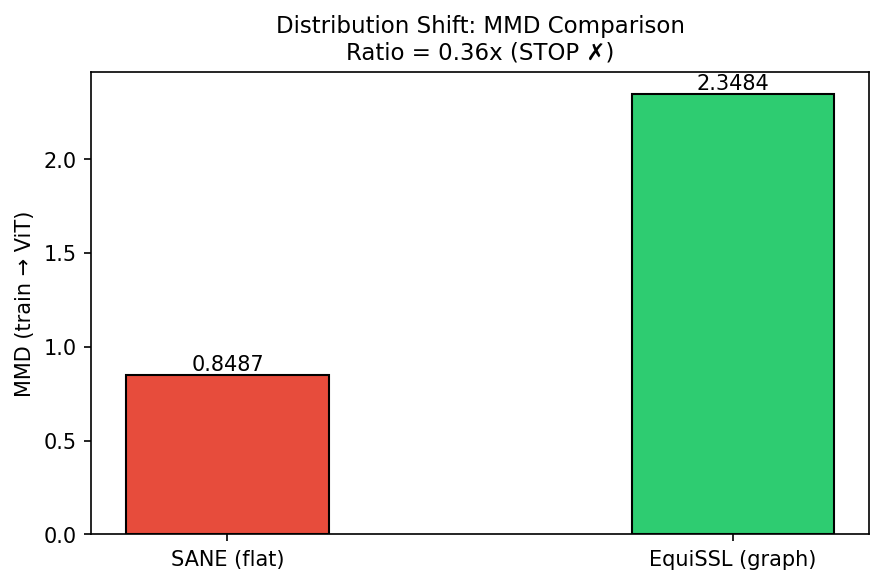
\includegraphics[width=0.5\linewidth]{figures/mmd_comparison.png}
  \caption{Cross-architecture MMD (CNN training zoo $\to$ ViT test zoo) for SANE and EquiSSL.}
  \label{fig:mmd_app}
\end{figure}

\section{Implementation Details}
\label{app:impl}

Full hyperparameter configurations are provided in Section~\ref{sec:method} and
Section~\ref{sec:setup}.
The validated optimal configuration (EquiSSL-perm, seed 0):

\begin{verbatim}
encoder:
  type: "neural-graphs (permutation equivariant)"
  hidden_dim: 256
  latent_dim: 128
  num_layers: 4
  symmetry: "permutation"  # NOT monomial

training:
  lr: 1.0e-3
  weight_decay: 1.0e-4
  batch_size: 64
  epochs: 100
  temperature: 0.07
  lambda_rec: 0.1
  scheduler: "CosineAnnealingLR(T_max=100, eta_min=1e-5)"

augmentation:
  perm_augment: true
  scale_augment: false  # Critical: do not use for ViT transfer

linear_probe:
  type: "RidgeCV"
  ridge_alphas: [0.1, 1.0, 10.0, 100.0]
  test_fraction: 0.2
\end{verbatim}

\emph{Note:} The EquiSSL (ScaleGMN) ablation encoder used in h-e1/h-m2 was trained for
50 epochs (vs.\ 100 epochs for EquiSSL-perm).
Future work should equalize epoch counts for a fully controlled ablation.
